\section{XG-PON Details} \label{section_xgpon}

The XG-PON standard  has many similarities with GPON, such as its
TDMA scheme used to share the medium, the mechanism to provide
QoS, and the DBA scheme used for the upstream wavelength. However,
some changes are required in order to support a larger number of
users, higher data rate, and extended physical reach. In this
section, we will present the details of XG-PON.


%Since LR-PON could pave the way for many exciting bandwidth
%intensive applications, FSAN of ITU has incorporated the key
%concepts of LR-PON into GPON and released XG-PON, the standard for
%the next generation optical access networks. This protocol has many
%similarities with GPON, such as its Time Division Multiple Access (TDMA)
%scheme used to share the medium and the mechanism to provide QoS.
%However, to exploit the benefits of LR-PON, the physical reach is increased
%from 20 km to 60 km, the downstream bandwidth is upgraded
%from 2.5 Gb/s to 10 Gb/s, and the maximum number of users
%per wavelength is increased from 64 to 256.
%In this section, we will present the details of XG-PON.


\subsection{Overview of XG-PON}

A series of recommendations has been released by FSAN of ITU-T for
XG-PON. ITU-T G.987 explains several important concepts of XG-PON
and ITU-T G.987.1 presents the general requirements, such as
network architecture, migration and coexistence with GPON,
services to be supported, hardware specifications, protocol stack,
etc. ITU-T G.987.2 focuses on issues of the physical media
dependent (PMD) layer, such as the used wavelength and the
supported data rates. ITU-T G.987.3 presents the details of
transmission convergence (TC) layer. Not only the protocols for
data communication, it also covers QoS management and Dynamic
Bandwidth Assignment (DBA) scheme for the upstream wavelength.
Another related recommendation is ITU-T G.988, which specifies ONU
management and control interface (OMCI) for both GPON and XG-PON.
Figure \ref{fig_xgpon_common_functions} illustrates XG-PON common
functions and the recommendations in which they are specified.


\begin{figure}[!htbp]
\begin{center}
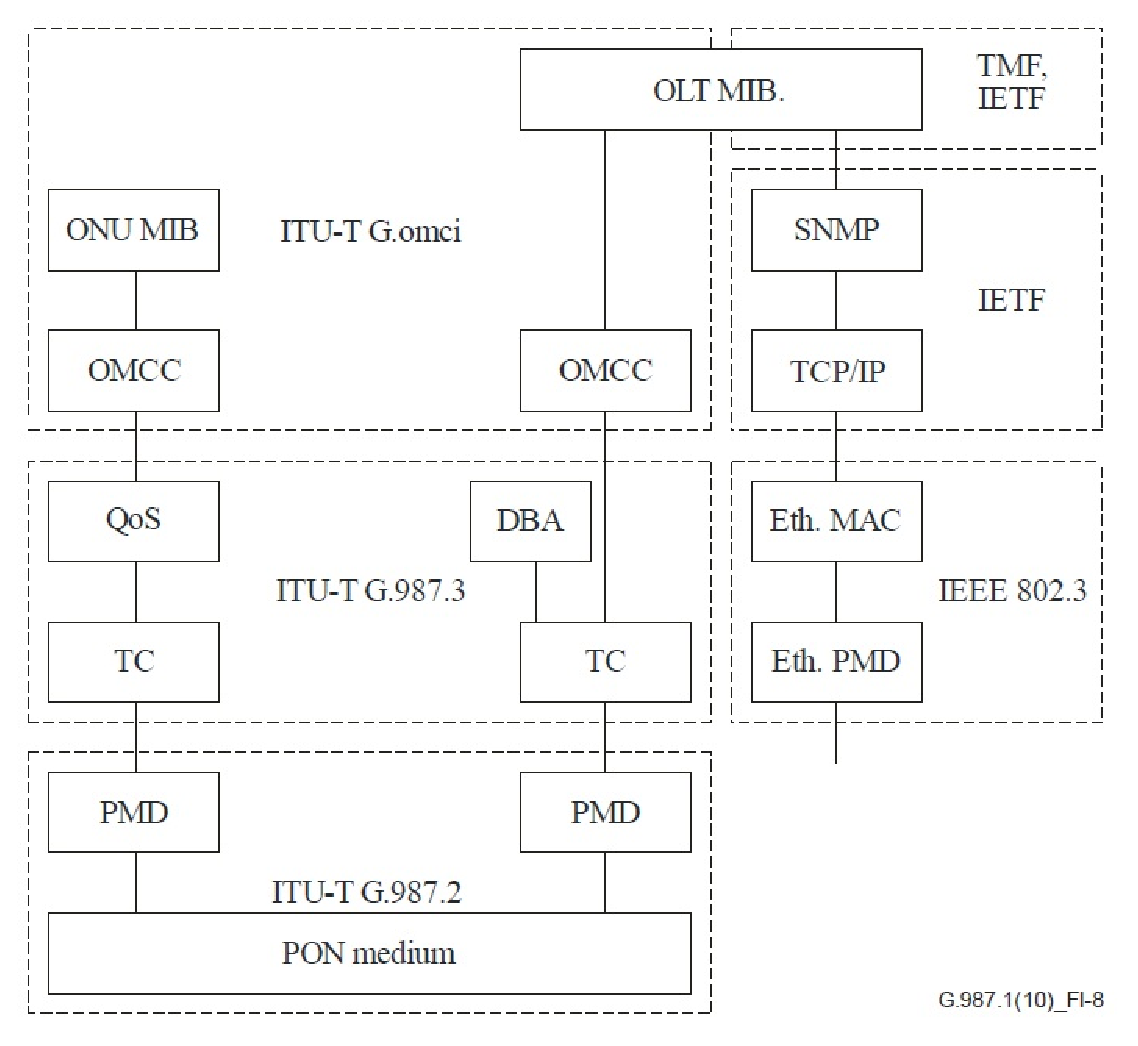
\includegraphics[width=0.6\textwidth]{images/xgpon_commonfunctions}
\end{center}
\vspace{-0.1in}
\caption{XG-PON common functions}
\label{fig_xgpon_common_functions}
\end{figure}





\subsection{Network Architecture}

XG-PON has been proposed for various deployment scenarios to serve
different customers, such as residential, business, and cell site.
To serve these customers, XG-PON lists the services to be
provided, such as Telephony, high speed Internet access, mobile
back-haul, etc. XG-PON also introduces many ONU variants that
provide different functions and interfaces. In summary, XG-PON has
been well standardized for providing full services to various
users with one optical network.



\begin{figure}[!htbp]
\begin{center}
\includegraphics[width=0.8\textwidth]{images/lrpon}
\end{center}
\vspace{-0.1in}
\caption{XG-PON Network Architecture} \label{fig_lrpon}
\end{figure}



As for optical distribution network, XG-PON can be deployed as a
classical PON, but mechanisms to extend its reach up to 60 km are
currently being defined. As illustrated in Figure \ref{fig_lrpon},
to support this longer physical reach, active component (Reach
Extender) can be applied in remote nodes and one XG-PON can be
composed of multiple passive segments connected through REs. These
REs can be optical amplifiers or optical-electrical-optical
regenerators that could fulfill the necessary optical link budget.




%As for optical distribution network, not only the classical PON network,
%XG-PON can also be deployed as a LR-PON network.
%As illustrated in Figure \ref{fig_lrpon}, passive optical splitters
%are still used for allowing multiple users to share optical fiber.
%To support long physical reach and large split ratio, Reach Extender (RE)
%can also be applied in remote nodes for fulfilling the necessary optical link budget.
%Hence, one XG-PON might be composed by multiple passive segments
%separated by REs.



\subsection{PMD Layer}
There are two flavours of XG-PONs based on the upstream line rate:
XG-PON1, featuring a 2.5 Gb/s upstream path, and XG-PON2,
featuring a 10 Gb/s one. The downstream line rate is 10 Gb/s in
both XG-PON1 and XG-PON2. ITU-T G.987.2 focuses on the PMD layer
for XG-PON1. XG-PON2 hasn't been standardized yet.

In XG-PON1, the used wavelengths are 1575-1580nm (downstream) and
1260-1280nm (upstream). The exact downstream line rate is 9.95328
Gb/s and the upstream one is 2.48832 Gb/s. For line coding, NRZ
(Non-Return to Zero)is used for both directions. ITU-T G.987.2
also specifies the requirements for hardwares, such as optical
fiber, transmitter/receiver, etc.





\subsection{Transmission Convergence Layer}


%For QoS management, XG-PON Transmission Convergence (XGTC) layer
%uses logical connections to carry traffic. QoS parameters of a
%connection are configured based on customer service level
%agreement. One unique XGEM port is used to identify a connection.
%To reduce the overhead of DBA scheme, the upstream XGEM ports are
%organized into Alloc-IDs. Note that XGEM ports of one Alloc-ID
%must belong to the same ONU. %Fundamentally, Alloc-ID is similar to
%the traffic container (T-CONT) in GPON.
The XG-PON Transmission Convergence (XGTC) layer is where the Medium
Access Control (MAC) protocol of XG-PON are defined.

To carry traffic between the OLT and the ONUs, the XGTC layer
maintains logical connections between these two entities,
designated XGEM Ports. Each connection is identified by a unique
XGEM Port-Id, which enables to send a packet to the correct ONU
and associate a connection to a certain Quality of Service (QoS)
agreement. Note that one connection is configured to carry
downstream or upstream traffics. It's impossible for two
connections in the same direction (downstream or upstream) to have
the same XGEM Port-Id, but one downstream connection may use the
same XGEM Port-Id with one upstream connection. To reduce the
overhead of the DBA scheme, upstream bandwidth is allocated to
groups of connections belonging to a single ONU. These groups are
designated as Transmission Containers (T-CONT) and each
group/T-CONT is identified by a unique identifier, the Alloc-Id.
Figure \ref{fig_multiplex} shows the multiplexing in XG-PON for
both directions.
%the upstream XGEM Ports
%are organized into groups of logical connections designated
%transmission containers (T-CONT). These T-CONTs are identified by
%unique Alloc-Ids and are used and .
%Depending on the type of traffic transported by the Alloc-Ids, these
%group of connections can be designated as transmission container (T-CONT),
%if it carries data traffic, or
%Note that XGEM Port-Ids of one Alloc-ID
%must belong to the same ONU.

%For QoS management, the XG-PON Transmission Convergence (XGTC) layer
%uses logical connections to carry traffic. These connections can
%have diferent QoS parameters and are identified through a unique
%XGEM Port-Id.
%QoS parameters of a
%connection are configured based on customer service level
%agreement. One unique XGEM port is used to identify a connection.
%To reduce the overhead of DBA scheme, the upstream XGEM Ports-Ids
%are organized into groups of logical connections idetified by Alloc-Ids.
%Note that XGEM Port-Ids of one Alloc-ID
%must belong to the same ONU. Fundamentally, Alloc-ID is similar to
%the traffic container (T-CONT) in GPON.

\begin{figure}[!htbp]
\begin{center}
\begin{tabular}{ccc}
\subfigure[{\small Downstream}]{\label{fig_multiplex:ds}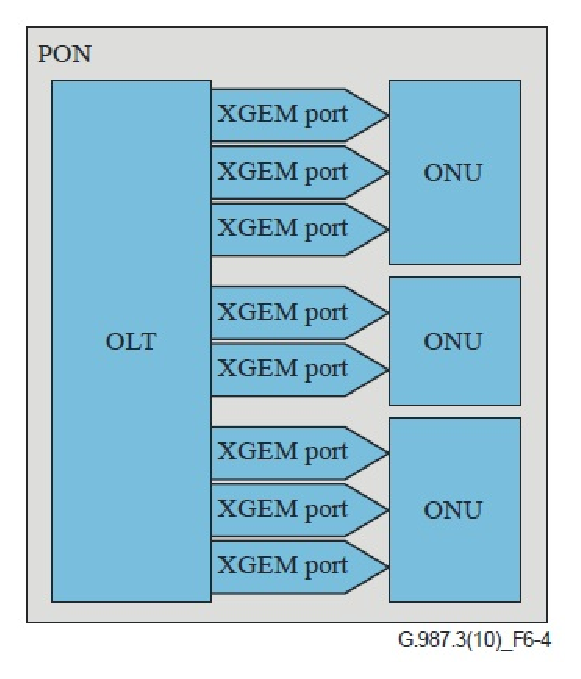
\includegraphics[width=0.36\textwidth]{images/ds_multiplex}} &  \hspace{0.1in} &
\subfigure[{\small Upstream}]{\label{fig_multiplex:us}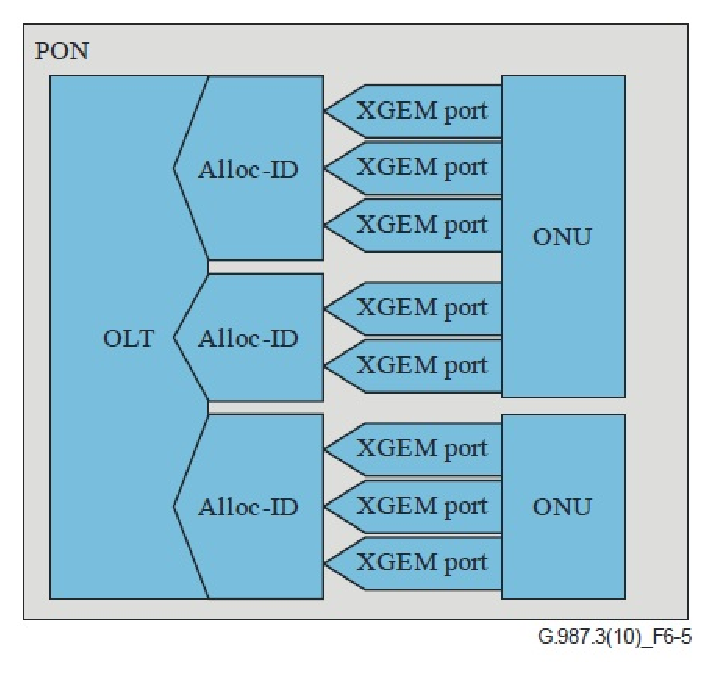
\includegraphics[width=0.45\textwidth]{images/us_multiplex}}
\end{tabular}
\end{center}
\vspace{-0.2in}
\caption{Multiplexing in XG-PON} \label{fig_multiplex}
\vspace{-0.1in}
\end{figure}

XGTC comprises three sublayers: service adaptation, framing, and
PHY adaptation, from top to bottom. Following these sublayers,
XGTC is introduced below.


\subsubsection{Service Adaptation Sublayer}

The service adaptation sublayer is responsible to adapt the upper
layer traffic to the transmission mechanisms of XG-PON. It will do
this by mapping upper layer traffic to the corresponding
connections, encapsulating/decapsulating data,
segmenting/reassembling SDUs when necessary and inserting padding
when there is not enough data to fill an XGTC frame. If needed, it
is also this sublayer's responsibility to encrypt/decrypt SDUs.

To map upper layer data to and from the connections of XGTC layer,
the OLT will maintain all connections and the ONU will maintain
the connections that belong to itself.


When the upper layer has something to transmit, it is also the
service adaptation sublayer's responsibility to select the
connections to be served according to their QoS parameters. When a
connection is scheduled to be served, the service adaptation
sublayer will then get data from its queue and insert an XGEM
header to create an XGEM frame. The XGEM header will contain an
XGEM Port-Id and some other information related to segmentation,
padding, encryption, etc.

When receiving an XGEM frame, the service adaptation sublayer will
get the XGEM Port-Id from the XGEM header. If the corresponding
connection exists in the connections maintained by the OLT/ONU,
this sublayer will carry out reassembly (if necessary) and pass
the data to upper layer. Otherwise, this XGEM frame will be
discarded.







%The service adaptation will insert the XGEM header

%Service adaptation sublayer interacts with upper layers directly.
%Each ONU will keep a list downstream and upstream XGEM Ports
%and it the Service Adaptation Layer responsibility to map data
%to this

%It is responsible to receive one Service Data Unit (SDU) from
%the upper layer, find the
%corresponding connection, and put this SDU into the queue of this
%connection. When this SDU is scheduled to transmit, this sublayer
%will encapsulate it into a XGEM frame and pass to framing
%sublayer. In case that this SDU is too large for the current
%transmission opportunity, it will be segmented. If needed, service
%adaptation sublayer is also responsible to encrypt this SDU.

%\footnote{In XG-PON, downstream traffic are broadcasted to all ONUs and must be encrypted to prevent eavesdropping. As for upstream traffic, encryption is optional.}.


%When one XGEM frame is received from framing sublayer, first


%based on
%XGEM port in the header, service adaptation sublayer first finds
%the corresponding connection. Decapsulation and the potential
%reassemble are then carried out. The resulting SDU will be
%dispatched to upper layer or OMCI client. Note that OMCI messages
%are treated as SDUs by XGTC layer and are carried by a special
%connection. If the SDU has been encrypted by the sender, this
%sublayer also carries out decryption. On ONU side, the service
%adaptation sublayer maintains the list of downstream XGEM ports
%for this ONU so that XGEM frames for other ONUs could be discarded
%directly.

%When one XGEM frame is received from framing sublayer, based on
%XGEM port in the header, service adaptation sublayer first finds
%the corresponding connection. Decapsulation and the potential
%reassemble are then carried out. The resulting SDU will be
%dispatched to upper layer or OMCI client. Note that OMCI messages
%are treated as SDUs by XGTC layer and are carried by a special
%connection. If the SDU has been encrypted by the sender, this
%sublayer also carries out decryption. On ONU side, the service
%adaptation sublayer maintains the list of downstream XGEM ports
%for this ONU so that XGEM frames for other ONUs could be discarded
%directly.


\subsubsection{Framing Sublayer}

In XG-PON, the OLT will send downstream XGTC frames every 125
$\mu$s, to broadcast traffic to all ONUs. In the upstream, ONUs
send variable length XGTC bursts to the OLT for their upstream
traffic. The length and start time of these upstream bursts are
determined by the OLT through a DBA algorithm.

The framing sublayer is responsible to generate and parse these
XGTC frames/bursts. When generating one downstream XGTC frame at
the OLT, the framing sublayer gets XGEM frames from service
adaptation sublayer and joins them together into an XGTC payload.
To create an upstream XGTC burst at ONU side, the framing sublayer
may create multiple XGTC payloads, where each payload will carry
XGEM frames from a single T-CONT. When parsing an XGTC
frame/burst, the framing sublayer will send its payloads to the
service adaptation sublayer for further processing.

In the header of the upstream XGTC burst generated by an ONU,
there might be queue occupancy reports for the T-CONTs of this
ONU. For each downstream XGTC frame, its header contains one
BW$_{map}$, which instructs ONUs to share the upstream wavelength
in a TDMA-like manner. More specifically, BW$_{map}$ specifies the
size of bandwidth allocations for T-CONTs, the used burst profile
(the length of preamble, the length of delimiter, forward error
correction or not, etc.), and the time to start to transmit. Since
the OLT-ONU physical distance could be quite different for ONUs,
each ONU should adjust the start time for avoiding collision in
the upstream direction. Note that when one ONU is activated, the
ranging procedure is carried out between the OLT and this ONU to
determine how to adjust the start time of its upstream bursts.
Figure \ref{fig_timelines} illustrates the time-lines in XG-PON.
The OLT and ONUs have a common view of the logic one-way delay of
the optical distribution network (the largest one-way propagation
delay plus various processing delay) and each ONU uses its own
equalization delay ($EqD$ calculated in ranging procedure) to
avoid collisions in upstream direction.

\begin{figure}[!htbp]
\begin{center}
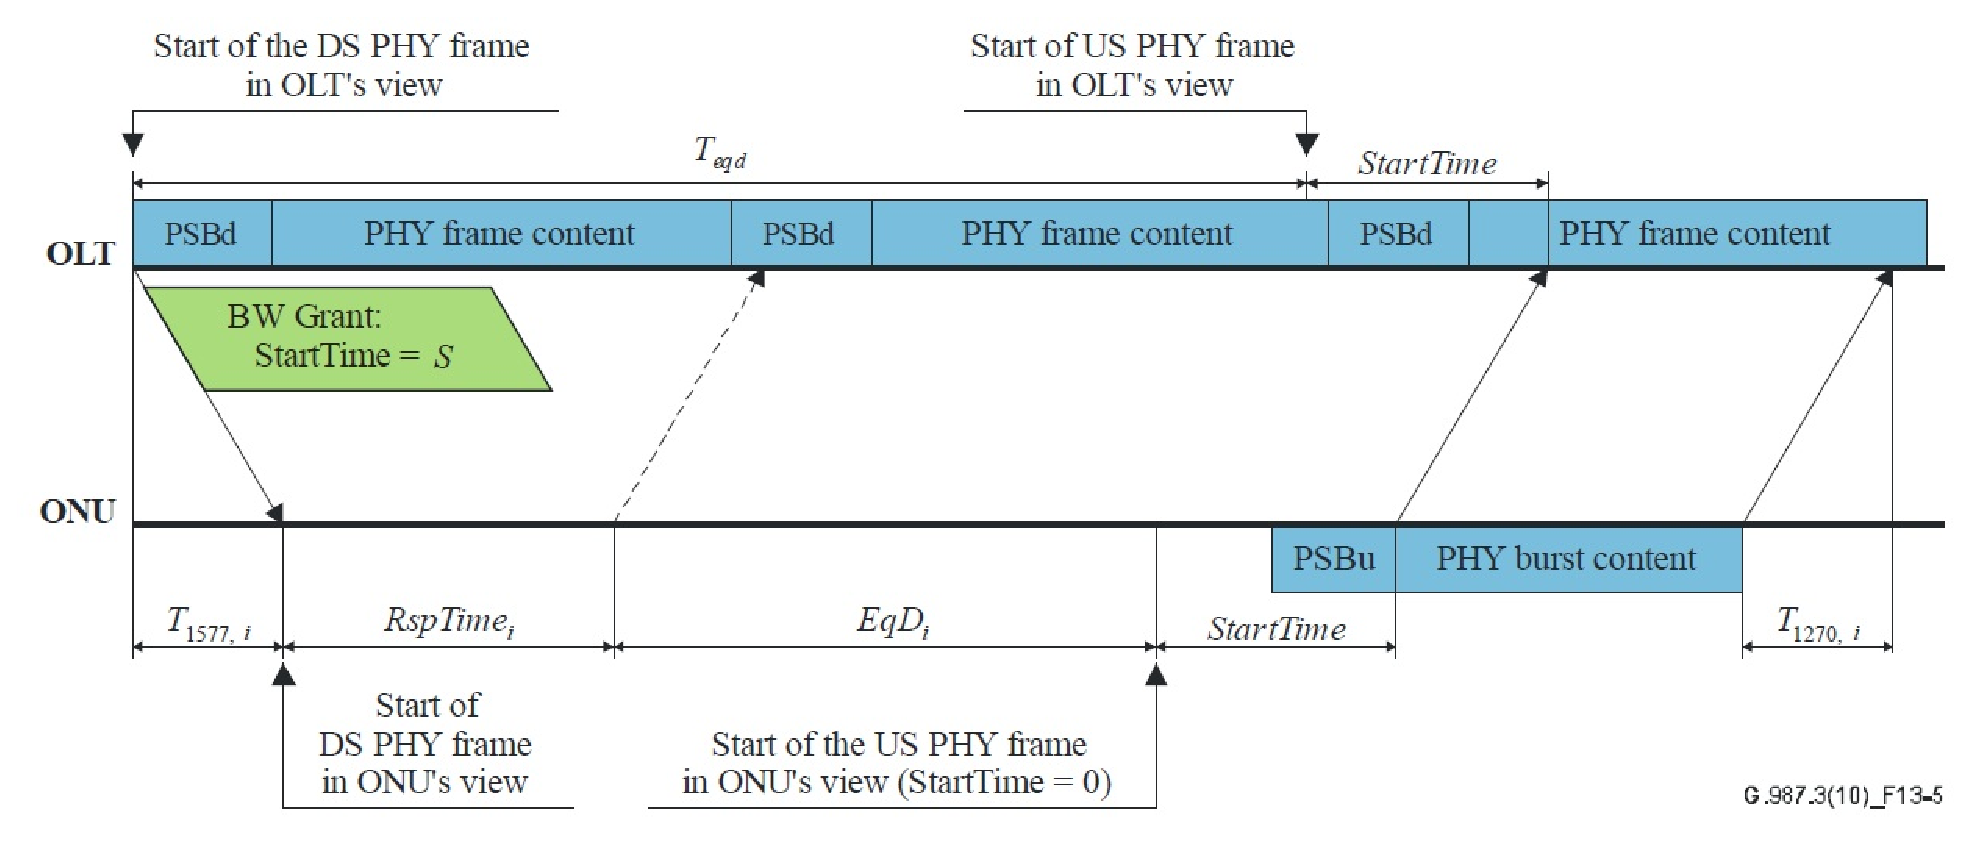
\includegraphics[width=0.9\textwidth]{images/xgpon_time}
\end{center}
\vspace{-0.1in}
\caption{Time-line in XG-PON} \label{fig_timelines}
\end{figure}


In the header of one upstream XGTC burst, the ONU can send one
PLOAM (Physical Layer Operations, Administration and Maintenance)
message to the OLT. As for one downstream XGTC frame, the OLT can
send multiple PLOAM messages to multiple ONUs. Through exchanging
PLOAM messages, many XGTC functions (key management, ONU power
management etc.) can be fulfilled.

\subsubsection{PHY Adaptation Sublayer}

PHY adaptation sublayer interacts with PMD layer directly. Its
main functions are forward error correction (FEC), scrambling, and
frame delineation through a Physical Synchronization Block (PSB).
In the downstream, the PHY adaptation sublayer will get an XGTC
frame to create a PHY frame. These PHY frames are sent
continuously every 125 $\mu$s. In the upstream, the PHY adaptation
sublayer will get the XGTC burst and create a PHY burst. These PHY
bursts have variable length due to the variable-length XGTC
bursts. In the PHY burst, the PSB is determined by a burst profile
selected by the OLT (through the BW$_{map}$) among the burst
profiles, that are configured through PLOAM messages.
\\
\\
Figure \ref{fig_sdumap} illustrates how these sublayers
encapsulate the SDUs of XG-PON into 125$\mu$s the downstream
frames or the variable-length upstream bursts.
\begin{figure}[!htbp]
\begin{center}
\begin{tabular}{ccc}
 \subfigure[{\small Downstream}]{\label{fig_sdumap:ds}\includegraphics[width=0.5\textwidth]{images/ds_sdumap}} &  \hspace{0.1in} &
\subfigure[{\small Upstream}]{\label{fig_sdumap:us}\includegraphics[width=0.435\textwidth]{images/us_sdumap}}
\end{tabular}
\end{center}
\vspace{-0.2in}
\caption{SDU Mapping in XG-PON} \label{fig_sdumap}
\vspace{-0.2in}
\end{figure}

%FEC (forward error correction) and scrambling
%for reliable data transmission. Physical synchronization block
%(PSB) is also added for frame delineation. In the upstream
%direction, PSB of one ONU's XGTC bursts are determined by the
%burst profile negotiated through PLOAM messages.
%Frame delineation is also carried out by this sublayer.


\subsection{Scheduling and DBA} \label{subsection_schedule_dba}

To decide the data to be transmitted in a downstream XGTC frame, a
downstream scheduler is used by the OLT. Based on QoS parameters
and service history of these downstream connections, the
downstream scheduler will decide the connections to be served and
the amount of data to be transmitted for each of them.

As for the upstream scheduling, the OLT uses a DBA algorithm to
allocate the upstream bandwidth to T-CONTs.  The DBA algorithm
makes decisions based on queue occupancy reports, QoS parameters,
and service history of these T-CONTs. The DBA algorithm needs to
select the T-CONTs to be served, reserve a short gap time between
the consecutive XGTC bursts for tolerating clock synchronization
errors, determine the size of each bandwidth allocation, and
calculate the start time for each bandwidth allocation. These
decisions are broadcast to ONUs through BW$_{map}$. Since the
upstream bandwidth is allocated to T-CONTs and each T-CONT may
have multiple upstream connections, the ONU also needs one
upstream scheduler to determine the upstream connections to be
served during one transmission opportunity assigned to one T-CONT.

These scheduling algorithms, especially the DBA algorithm, are
very important to network performance and QoS management. To allow
competition and encourage research, these algorithms were
intentionally left out of the standard. Indeed, it has been a very
hot topic to study DBA algorithms for EPON and GPON
\cite{han08dba4gpon}\cite{leligou06GiantMACforGPON}\cite{song09multithread4LRPON}.
Hence, there should be many research opportunities for XG-PON too.
